\documentclass[11pt]{article}
\usepackage[T1]{fontenc}
\usepackage[utf8]{inputenc}
\usepackage{lmodern}
\usepackage[a4paper,margin=28mm]{geometry}
\usepackage{amsmath,amssymb,amsthm,mathtools}
\usepackage{microtype}
\usepackage{booktabs}
\usepackage{tikz}
\usetikzlibrary{arrows.meta,positioning}
\usepackage{xcolor}
\definecolor{linkblue}{RGB}{24,65,105}
\usepackage[colorlinks=true,allcolors=linkblue,breaklinks=true]{hyperref}
\usepackage[capitalise,noabbrev]{cleveref}
\hypersetup{
  pdftitle={Lipschitz Equivalent Separable Banach Spaces Need Not Be Linearly Isomorphic},
  pdfauthor={OpenAI}
}
\newcommand{\R}{\mathbb R}
\newcommand{\N}{\mathbb N}
\newcommand{\F}{\mathcal F}
\DeclareMathOperator{\Lip}{Lip}
\DeclareMathOperator{\dist}{dist}
\DeclareMathOperator{\supp}{supp}
\DeclareMathOperator{\spanlin}{span}
\newtheorem{theorem}{Theorem}[section]
\newtheorem{proposition}[theorem]{Proposition}
\newtheorem{lemma}[theorem]{Lemma}
\newtheorem{corollary}[theorem]{Corollary}
\theoremstyle{definition}
\newtheorem{definition}[theorem]{Definition}
\theoremstyle{remark}
\newtheorem{remark}[theorem]{Remark}
\numberwithin{equation}{section}
\allowdisplaybreaks[2]
\setlength{\emergencystretch}{2em}

\title{Lipschitz Equivalent Separable Banach Spaces\\
Need Not Be Linearly Isomorphic}
\author{OpenAI}
\date{September 24, 2026}

\begin{document}
\maketitle
\begin{abstract}
There are separable real Banach spaces that are globally bi-Lipschitz
equivalent but not linearly isomorphic. This gives a negative answer
to the separable Banach-space Lipschitz-isomorphism problem.
\end{abstract}

\section{Introduction}
\label{sec:introduction}

A Banach-space norm defines both a linear topology and a metric.
A bounded linear isomorphism preserves the metric up to multiplicative
constants, but a map with that metric property need not preserve
addition or scalar multiplication. The Lipschitz-isomorphism problem
asks whether a \emph{bijection} with two-sided Lipschitz bounds nevertheless
forces two Banach spaces to be linearly isomorphic. We consider the
separable real case and obtain a negative answer.

Throughout, \(\ell_2\) denotes the real separable Hilbert space of
square-summable scalar sequences. For a Banach space \(H\), set
\[
 c_0(H)=\{(v_i)_{i\ge1}:v_i\in H,\ \|v_i\|\longrightarrow0\},
 \qquad \|(v_i)\|=\sup_i\|v_i\|.
\]
Ordinary \(c_0\) means \(c_0(\R)\). A linear embedding means a bounded
linear map that is bounded below; its range is consequently closed.

\begin{theorem}
\label{thm:main}
There are separable real Banach spaces \(X,Y\) and a bijection
\(\Psi:X\to Y\) such that, for every \(s,t\in X\),
\begin{equation}
\label{eq:main-bounds}
 \frac4{21}\|s-t\|_X
 \le \|\Psi(s)-\Psi(t)\|_Y
 \le \frac{76}{25}\|s-t\|_X.
\end{equation}
The space \(X\) contains a linearly isometric copy of \(c_0(\ell_2)\), while
\(Y\) contains no closed subspace linearly isomorphic to
\(c_0(\ell_2)\). In particular, \(X\) and \(Y\) are not linearly
isomorphic.
\end{theorem}

The obstruction in this theorem is deliberately block-valued:
each coordinate of \(c_0(\ell_2)\) is an entire Hilbert space.
It does not say that \(Y\) contains no ordinary \(c_0\).
The Hilbert block in each coordinate is essential to the obstruction
proved below.

\subsection*{Historical setting}

Ribe proved that uniformly homeomorphic normed spaces have the same
finite-dimensional linear structure up to a uniform distortion bound
\cite[Theorem~1]{Ribe76}. That result shows how much linear information
can survive even a weaker form of metric equivalence. At the same time,
Aharoni and Lindenstrauss constructed Lipschitz equivalent,
nonisomorphic nonseparable Banach spaces and explicitly asked for
separable examples \cite[pp.~281--282]{AL78}. Ribe later constructed
separable uniformly homeomorphic, nonisomorphic spaces \cite{Ribe84}.
Aharoni and Lindenstrauss then gave uniform pairs that are not
Lipschitz equivalent \cite{AL85}, while Johnson, Lindenstrauss and
Schechtman developed further separable uniform examples and left the
separable Lipschitz question open
\cite[Theorem~5.8 and Section~8(3)]{JLS96}. These developments make the
global two-sided estimate in \eqref{eq:main-bounds} a substantive
requirement, rather than a reformulation of a uniform counterexample.

Several positive results explain why the separable question resists a
direct transfer of those examples. Godefroy, Kalton and Lancien proved
that a Banach space Lipschitz isomorphic to \(c_0\) is linearly
isomorphic to \(c_0\), and that being linearly isomorphic to a subspace
of \(c_0\) is invariant under Lipschitz isomorphism
\cite[Theorems~2.1--2.2]{GKL00}. Godefroy and Kalton's lifting theorem
places every separable Banach space linearly and isometrically inside
its Lipschitz-free space; their quotient corollary converts a
Lipschitz right inverse of a linear quotient onto a separable space
into a bounded linear right inverse
\cite[Theorem~3.1 and Corollary~3.2]{GK03}. The construction below uses
free spaces; \Cref{rem:no-section} explains the distinction between
the lift used here and a right inverse of the linearized correction.

In the quasi-Banach setting, Albiac and Kalton obtained separable
counterexamples for every \(0<p<1\) \cite[Theorem~5.4]{AK09}.
The strict inequality \(p<1\) is part of that theorem, so it does not
settle the Banach-norm case. Kalton recorded the separable
Lipschitz-isomorphism question as Problem~3 in his 2008 survey
\cite[Section~2.2]{Kalton08}; Albiac, Ansorena, B\'{i}ma and C\'{u}th
still described the Banach case as open in the first paragraph of
their paper published online in December 2025 \cite{AABC26}.
Theorem~\ref{thm:main} resolves that question negatively for separable
real Banach spaces. It asserts neither reflexivity nor a complex-scalar
analogue.

For comparison, every surjective isometry between the unit spheres of
nonzero real Banach spaces extends uniquely to a surjective real-linear
isometry \cite[Theorem~1.1]{OpenAITingley}.
That result concerns exact distances on unit spheres; here we allow
fixed multiplicative distortion but require a bijection of the whole
spaces.

\subsection*{Proof overview}

The proof separates the metric construction from the linear
obstruction. Its intermediate map acts between Hilbert spaces:
\[
 M=U\oplus_2 V,\qquad V=\ell_2,\qquad
 h:M\longrightarrow U.
\]
Here \(U=(\bigoplus_{n\ge1}U_n)_2\) is a Hilbert sum of
finite-dimensional coordinate blocks. The map \(h\) is an onto
bi-Lipschitz change of variables fixing zero, close to an isometry. Its relevant
nonlinear part is
\[
 D(u,v)=h(u,v)-u.
\]
The construction arranges that, near any finite family of distinct
points of \(M\), the sufficiently high output coordinates of \(D\)
lie in mutually orthogonal coordinate subspaces. The cutoff index and
the neighborhoods may depend on that finite family. We call this
property \emph{local orthogonality}.

To turn this geometry into a linear obstruction, use the
Lipschitz-free space \(E=\F(M)\), the closed linear span of evaluation
functionals on real zero-preserving Lipschitz functions.
The evaluation map \(\delta:M\to E\) preserves distances. Every
zero-preserving Lipschitz map has a bounded linearization, so \(D\)
determines \(q:E\to U\) by
\[
 q\delta(u,v)=h(u,v)-u.
\]
Section~\ref{sec:localization} proves that local orthogonality makes
\(q\) \emph{completely continuous}: a weakly null sequence in \(E\)
has norm-null image. This is the one place where the local coordinate
geometry enters the Banach-space obstruction.

The linearization is also what makes the metric change of variables
possible. Give \(E\oplus V\) its sum norm and put
\[
 Q_1(e,v)=(qe,v),\qquad
 B(e,v)=e+\delta(qe,v).
\]
The identity \(qB=hQ_1\) is triangular: applying \(q\) to the new
variable records \(h\) of the old output. Given \(z\in E\), one first
recovers \(x=h^{-1}(qz)\) and then subtracts \(\delta(x)\); this yields
the explicit inverse of \(B\). Section~\ref{sec:triangular} proves
both inverse identities and keeps track of the sum norm.

For a bounded linear \(Q:A\to H\), the graph space used in the final
step consists of sequences \(s=(s_i)\) for which
\(\sum_i2^{-i}\|s_i\|<\infty\) and \((Qs_i)\in c_0(H)\), with norm
\[
 \|s\|_{Z_Q}
 =\max\left\{\sum_i2^{-i}\|s_i\|,\ \sup_i\|Qs_i\|\right\}.
\]
Set \(X=Z_{Q_1}\) and \(Y=Z_q\). Applying \(B\) in each coordinate
gives the desired bijection: \(qB=hQ_1\) controls the second part of
the graph norm, and the Lipschitz bounds for \(B\) control the weighted
sum. The \(V\) coordinates embed \(c_0(V)\) isometrically in \(X\).
By contrast, complete continuity of \(q\) makes each fixed output
coordinate tend to zero along an orthonormal sequence in any Hilbert
block of a proposed \(c_0(\ell_2)\) copy in \(Y\).
A disjoint-support argument then finds a unit vector in each block
with arbitrarily small full \(c_0(U)\) output. A surviving copy would embed
ordinary \(c_0\) into \(\ell_1(E)\). Section~\ref{sec:free-graph}
excludes this because \(E=\F(M)\) is weakly sequentially complete.

Two analytic steps supply the inputs just described. For localized
linearization, a hypothetical non-null image of a weakly null
sequence produces uniformly Lipschitz scalar tests \(d_i\).
Orthogonality allows only finitely many points where their limiting
local Lipschitz constants remain large. Cutoffs remove neighborhoods
of those points; a shrinking-ball lemma shows that the removed tests
pair negligibly with the weakly null sequence. The compact reduction
theorem of Aliaga, No\^us, Petitjean and Proch\'azka
\cite[Theorem~2.3]{ANPP21} then reduces the remainder to a compact set,
where a finite cover controls its Lipschitz constant.

For the Hilbert map, a unit vector in each block is designated as a
slot. With the slots frozen, perpendicular components stay in their
blocks, old slot coordinates move to even blocks, and the additional
\(\ell_2\) coordinates fill odd blocks. This is an onto linear
isometry. The slots are then allowed to depend on the input so that
near different points they eventually use disjoint coordinates.
Finite approximants freeze all but finitely many slots and have
uniform global inverse bounds. Section~\ref{sec:hilbert} constructs the slots with a common radial
derivative budget, proves global invertibility of the finite approximants,
and passes to an onto limit. Its decisive estimate bounds every tail of the
inverse images by the corresponding tail of a fixed output, with an
exact cancellation of slot terms. Section~\ref{sec:assembly} combines
the results and computes the constants in \eqref{eq:main-bounds}.

\section{Free spaces and the graph-space obstruction}
\label{sec:free-graph}

The metric construction will provide a bounded linear operator
\(q:E\to U\) that is completely continuous, with \(E\) weakly
sequentially complete. This section explains why those two properties
exclude \(c_0(\ell_2)\) from the associated graph space. We first
record the free-space facts that produce \(E\), then prove the
obstruction without assuming compactness of any operator into
\(c_0(U)\).

\subsection{Free-space facts and the two external inputs}

For a pointed metric space \((M,d,0)\), let \(\Lip_0(M)\) be the
Banach space of real Lipschitz functions \(f:M\to\R\) with \(f(0)=0\),
normed by \(\Lip(f)\). Let \(\delta(x)\in\Lip_0(M)^*\) be evaluation
at \(x\), and define
\[
 \F(M)=\overline{\spanlin}\{\delta(x):x\in M\}
       \subset\Lip_0(M)^*.
\]
The evaluation and molecule construction goes back to Arens and Eells
\cite[Sections~2--3]{AE56}; the notation here is the later
Lipschitz-free formulation. In particular, \(\delta(0)=0\).
When a Lipschitz function \(f\) need not vanish at \(0\), the pairing
\(\langle f,\mu\rangle\) means \(\langle f-f(0),\mu\rangle\).

The evaluation map preserves distances:
\begin{equation}
\label{eq:delta-isometry}
 \|\delta(x)-\delta(y)\|=d(x,y).
\end{equation}
The Lipschitz inequality gives the upper bound. For the reverse bound,
test against \(t\mapsto d(t,y)-d(0,y)\), which has Lipschitz constant
at most one. If \(M\) is separable, choose a countable dense set
\(D_0\subset M\). Equation~\eqref{eq:delta-isometry} shows that finite
rational linear combinations of \(\delta(D_0)\) are dense in
\(\F(M)\); hence \(\F(M)\) is separable.

If \(K\subset M\) contains \(0\), the closed span of \(\delta(K)\)
in \(\F(M)\) is isometric to \(\F(K)\). To see this, a real
\(L\)-Lipschitz function \(f\) on \(K\) extends with the same
Lipschitz constant by the McShane formula
\cite[Lemma~3.1 and the following paragraph]{Kalton04}
\[
 \widetilde f(x)=\inf_{z\in K}\bigl(f(z)+L\,d(x,z)\bigr).
\]
For \(L=0\) use the constant extension. For \(L>0\), the Lipschitz
inequality on \(K\) makes the displayed infimum equal to \(f\) there,
and the triangle inequality gives the \(L\)-Lipschitz bound on \(M\).
The infimum is finite because \(0\in K\) supplies an upper bound and
the triangle inequality supplies a lower bound. Thus the suprema
defining the two free-space norms agree on finite evaluation sums
supported in \(K\), and then on their closures. In particular,
\begin{equation}
\label{eq:compact-pairing}
 |\langle f,\nu\rangle|
 \le \Lip(f|_K)\|\nu\| \qquad(\nu\in\F(K)).
\end{equation}

For any Banach space \(H\) and any Lipschitz map \(D:M\to H\) with
\(D(0)=0\), there is a unique bounded linear map
\begin{equation}
\label{eq:linearization}
 \widehat D:\F(M)\to H,\qquad
 \widehat D\delta(x)=D(x),\qquad
 \|\widehat D\|=\Lip(D).
\end{equation}
Indeed, for a finite evaluation sum, define
\(\widehat D(\sum_j a_j\delta(x_j))=\sum_j a_jD(x_j)\).
Testing the latter vector against a norm-one functional in \(H^*\)
and using the free-space norm gives
\[
 \left\|\sum_j a_jD(x_j)\right\|
 \le \Lip(D)\left\|\sum_j a_j\delta(x_j)\right\|.
\]
This inequality makes the definition independent of the chosen
representation and extends it continuously to \(\F(M)\).
Testing the extension on \(\delta(x)-\delta(y)\) proves the reverse
norm bound. This metric-domain linearization is recorded in
\cite[Lemma~3.2]{Kalton04}; for Banach-space domains see also
Godefroy and Kalton \cite[Lemma~2.5]{GK03}.

A bounded linear operator is \emph{completely continuous} if it sends
each weakly null sequence to a norm-null sequence. A Banach space is
\emph{weakly sequentially complete} if each weakly Cauchy sequence
has a weak limit in the space. We use the following two external
results with exactly the displayed hypotheses.

\begin{theorem}[Compact reduction for a weakly null sequence]
\label{thm:compact-reduction}
Let \((M,d,0)\) be a complete pointed metric space, and let
\(\mu_i\to0\) weakly in \(\F(M)\). For every \(\tau>0\), there is a
compact \(K\subset M\), with \(0\in K\), such that
\[
 \dist(\mu_i,\F(K))<\tau\qquad\hbox{for every }i.
\]
\end{theorem}

This is the sequential consequence of the tightness theorem of
Aliaga, No\^us, Petitjean and Proch\'azka
\cite[Theorem~2.3, arXiv version cited in the bibliography]{ANPP21}.
Their theorem states that every weakly precompact subset \(W\) of
\(\F(M)\), for complete \(M\), is tight: for each \(\epsilon>0\)
there is compact \(K_0\subset M\) with
\(W\subset\F(K_0)+\epsilon B_{\F(M)}\), where for an arbitrary
subset \(K_0\) this notation means its closed evaluation span inside
\(\F(M)\).
Here weak precompactness means that every sequence in \(W\) has a
weakly Cauchy subsequence. The set \(\{0,\mu_1,\mu_2,\ldots\}\)
has that property: any sequence in it has either a constant
subsequence or a subsequence whose indices tend to infinity, which
converges weakly to zero. Apply the theorem with \(\epsilon=\tau/2\)
and enlarge \(K_0\) by \(0\). This gives the strict inequality above.
Kalton's finite-radius localization lemma
\cite[Lemma~4.5]{Kalton04} is a precursor to this complete-space
compact reduction.

\begin{theorem}[Weak sequential completeness of a free space]
\label{thm:free-wsc}
If \(M\) is a superreflexive real Banach space, then \(\F(M)\) is
weakly sequentially complete. In particular, this applies to every
real Hilbert space \(M\).
\end{theorem}

This is \cite[Corollary~2.5, arXiv version cited in the
bibliography]{ANPP21}. Its compact-set input is the Main Theorem of
Kochanek and Perneck\'a \cite{KP18}, which concerns free spaces over
compact subsets of superreflexive Banach spaces, not directly the
whole Hilbert space.

\subsection{Weighted graph spaces}

Let \(A,H\) be real Banach spaces and \(Q:A\to H\) bounded
and linear. Define
\begin{align}
\label{eq:graph-space}
 Z_Q=\bigl\{s=(s_i)_{i\ge1}:{}&
 s_i\in A,\quad \sum_{i\ge1}2^{-i}\|s_i\|<\infty,\quad
 (Qs_i)_{i\ge1}\in c_0(H)\bigr\},\\
\label{eq:graph-norm}
 \|s\|_{Z_Q}
 ={}&\max\left\{\sum_{i\ge1}2^{-i}\|s_i\|,
                         \sup_{i\ge1}\|Qs_i\|\right\}.
\end{align}
The membership condition is part of the definition; finiteness of the
displayed maximum alone would not require the \(Q\)-images to tend to
zero.

\begin{lemma}
\label[lemma]{lem:graph-banach}
\(Z_Q\) is a Banach space, and it is separable if \(A,H\) are
separable. The coordinate map
\(p_i:Z_Q\to A\), \(p_i(s)=s_i\), has norm at most \(2^i\), and
\[
 J_Q:Z_Q\to c_0(H),\qquad J_Q(s)=(Qs_i)_i,
\]
has norm at most one.
\end{lemma}

\begin{proof}
Let \(\ell_1(2^{-i};A)\) denote the weighted sum space with norm
\(\sum_i2^{-i}\|s_i\|\). The map \(s\mapsto(2^{-i}s_i)_i\)
is an isometry from this space onto \(\ell_1(A)\), so it is complete.
The map
\[
 s\longmapsto \bigl(s,(Qs_i)_i\bigr)
\]
identifies \(Z_Q\) isometrically with a subspace of
\(\ell_1(2^{-i};A)\oplus_\infty c_0(H)\). This subspace is closed.
In fact, suppose \((s^{(k)},(Qs_i^{(k)})_i)\) converges there to
\((s,y)\). For each fixed \(i\),
\[
 \|s_i^{(k)}-s_i\|
 \le 2^i\|s^{(k)}-s\|_{\ell_1(2^{-j};A)}
 \longrightarrow0.
\]
Continuity of \(Q\) gives \(Qs_i^{(k)}\to Qs_i\), whereas convergence
in \(c_0(H)\) gives \(Qs_i^{(k)}\to y_i\). Thus \(y_i=Qs_i\) for all
\(i\), as required. Completeness follows.

If \(A,H\) are separable, truncating a sequence in \(Z_Q\) gives
convergence in both parts of
\eqref{eq:graph-norm}: the weighted sum has a vanishing tail, and the
\(Q\)-image is norm-null. Choose a fixed countable dense subset of
\(A\). The finitely supported sequences with entries in that subset
form a countable dense subset of \(Z_Q\), because each of their
finitely many entries may be approximated in \(A\) and \(Q\) is
continuous. Finally, the two claimed operator bounds are immediate
from \eqref{eq:graph-norm}.
\end{proof}

The next lemma records exactly the consequence of weak sequential
completeness that the graph obstruction needs. It does not assert
that every operator into a \(c_0\)-sum is compact.

\begin{lemma}
\label[lemma]{lem:no-c0-sum}
If \(E\) is a weakly sequentially complete real Banach space, then
\(\ell_1(E)\) contains no closed subspace linearly isomorphic to
ordinary \(c_0\).
\end{lemma}

\begin{proof}
Every finite direct sum of \(E\) is weakly sequentially complete:
the coordinates of a weakly Cauchy sequence are weakly Cauchy in
\(E\), hence have weak limits, and the finite list of limits is the
weak limit in the sum. The property also passes to a closed linear
subspace \(F\) of a weakly sequentially complete space \(G\).
Indeed, a weakly Cauchy sequence in \(F\) is weakly Cauchy in \(G\);
its weak limit lies in \(F\), since a closed linear subspace is
weakly closed by Hahn--Banach separation. Every functional on \(F\)
extends to \(G\) by Hahn--Banach, so the same limit is weak in \(F\).

Ordinary \(c_0\) is not weakly sequentially complete. If
\((e_k)\) is its usual unit basis, the partial sums
\(e_1+\cdots+e_n\) are weakly Cauchy: for every
\((a_k)\in c_0^*=\ell_1\), their pairings are the Cauchy partial sums
\(\sum_{k\le n}a_k\). A weak limit would have every coordinate equal
to one, which is not an element of \(c_0\).

Suppose now that \(A:c_0\to\ell_1(E)\) is a linear embedding with
\(\|Ax\|\ge b\|x\|\), where \(b>0\). Let \(P_N\) be projection onto
the first \(N\) coordinates, with \(P_0=0\). No \(P_NA\) is bounded
below, because otherwise its closed range would be a copy of \(c_0\)
in the weakly sequentially complete finite sum \(E^N\).

Starting with \(N_0=0\), choose unit vectors \(x_j\in c_0\) and
integers \(N_j>N_{j-1}\) recursively so that
\[
 \|P_{N_{j-1}}Ax_j\|<b/8,\qquad
 \|(I-P_{N_j})Ax_j\|<b/8.
\]
The first inequality is possible because \(P_{N_{j-1}}A\) is not
bounded below; after choosing \(x_j\), its \(\ell_1(E)\) tail gives
the second. Put \(z_j=(P_{N_j}-P_{N_{j-1}})Ax_j\). Then
\[
 \|Ax_j-z_j\|<b/4,\qquad \|z_j\|>3b/4.
\]
The \(z_j\) have disjoint coordinate supports. For any finite scalar
family \((\alpha_j)\),
\begin{align*}
 \left\|\sum_j\alpha_jAx_j\right\|
 &\ge \left\|\sum_j\alpha_jz_j\right\|
       -\sum_j|\alpha_j|\|Ax_j-z_j\|\\
 &=\sum_j|\alpha_j|\|z_j\|
       -\sum_j|\alpha_j|\|Ax_j-z_j\|
 \ge \frac b2\sum_j|\alpha_j|.
\end{align*}
Consequently,
\[
 \frac{b}{2\|A\|}\sum_j|\alpha_j|
 \le\left\|\sum_j\alpha_jx_j\right\|_{c_0}
 \le\sum_j|\alpha_j|.
\]
The finite-sum map therefore extends by completeness to a bounded
linear embedding of \(\ell_1\) into \(c_0\), with closed range.
This is impossible. If \(F\) is any closed subspace of \(c_0\), the
restriction map \(c_0^*=\ell_1\to F^*\) is onto by Hahn--Banach,
so \(F^*\) is separable. A subspace isomorphic to \(\ell_1\) would
instead have dual isomorphic to \(\ell_\infty\), which is
nonseparable: the uncountable set of all \(0\)-\(1\) sequences is
pairwise separated by distance one. This contradiction proves the
lemma.
\end{proof}

\begin{lemma}
\label[lemma]{lem:graph-obstruction}
Let \(E,U\) be real Banach spaces, with \(E\) weakly sequentially
complete, and let \(q:E\to U\) be a completely continuous bounded
linear operator.
Then \(Z_q\) contains no closed subspace linearly isomorphic to
\(c_0(\ell_2)\).
\end{lemma}

\begin{proof}
Suppose that \(S:c_0(\ell_2)\to Z_q\) is a linear embedding with
\(\|Sx\|_{Z_q}\ge b_0\|x\|\), \(b_0>0\).
We will select a scalar copy of \(c_0\) on which the \(c_0(U)\)
part of \(S\) has norm at most \(b_0/2\). The weighted sum part of
the graph norm must then retain the lower bound \(b_0\), giving a
copy of \(c_0\) in \(\ell_1(E)\), contrary to
\Cref{lem:no-c0-sum}.

Write
\(I_n:\ell_2\to c_0(\ell_2)\) for injection into the \(n\)th
coordinate and put
\[
 T_n=J_qSI_n:\ell_2\to c_0(U).
\]
We first prove that each \(T_n\) fails to be bounded below.

Fix \(n\) and an orthonormal sequence \((e_k)\) in \(\ell_2\).
It is weakly null, since the scalar coefficients of a fixed Hilbert
vector against an orthonormal sequence are square summable. For each
fixed \(i\), boundedness of \(p_iSI_n\) therefore gives
\(p_iSI_ne_k\to0\) weakly in \(E\). Complete continuity of \(q\)
implies
\[
 \|(T_ne_k)_i\|=\|q\,p_iSI_ne_k\|\longrightarrow0
 \qquad\hbox{for each fixed }i.
\]
Set \(y_k=T_ne_k\), so \(\|y_k\|\le\|T_n\|\).
Choose \(k_j\) increasing and integers
\(0=m_0<m_1<m_2<\cdots\) as follows. Having chosen \(m_{j-1}\),
choose \(k_j\) so large that
\[
 \max_{i\le m_{j-1}}\|(y_{k_j})_i\|<2^{-j}.
\]
The maximum over no coordinates is zero. Then choose \(m_j>m_{j-1}\)
so large that \(\sup_{i>m_j}\|(y_{k_j})_i\|<2^{-j}\), using
\(y_{k_j}\in c_0(U)\). Let \(z_j\) be the restriction of \(y_{k_j}\)
to coordinates \(m_{j-1}<i\le m_j\). Thus
\[
 \|y_{k_j}-z_j\|<2^{-j},\qquad \|z_j\|\le\|T_n\|.
\]
Because the \(z_j\) have disjoint coordinate supports, for all \(N\)
\[
 \left\|\sum_{j=1}^N T_ne_{k_j}\right\|
 \le \left\|\sum_{j=1}^N z_j\right\|
          +\sum_{j=1}^N2^{-j}
 \le \|T_n\|+1.
\]
The corresponding input sum has Hilbert norm \(\sqrt N\).
No positive lower bound for \(T_n\) is compatible with these two
estimates.

Choose a unit vector \(t_n\in\ell_2\) such that
\(\|T_nt_n\|\le b_0\,2^{-n-1}\). The map
\[
 R:c_0\to c_0(\ell_2),\qquad R(a)=(a_nt_n)_n
\]
is a linear isometry. For finitely supported \(a\),
\[
 \|J_qSRa\|
 \le\sum_n |a_n|\|T_nt_n\|
 \le\frac{b_0}{2}\|a\|_\infty.
\]
Truncation in \(c_0\) and continuity extend this estimate to every
\(a\in c_0\). On the other hand
\(\|SRa\|_{Z_q}\ge b_0\|a\|_\infty\).
The second part of the maximum in \eqref{eq:graph-norm} is at most
\((b_0/2)\|a\|_\infty\), so the first part must satisfy
\[
 \sum_i2^{-i}\|(SRa)_i\|\ge b_0\|a\|_\infty.
\]
For \(a=0\) this is immediate; for \(a\ne0\) it follows because the
second part is strictly below the required lower bound for the
maximum. Hence
\[
 a\longmapsto \bigl(2^{-i}(SRa)_i\bigr)_i
\]
is a bounded linear embedding of \(c_0\) into \(\ell_1(E)\).
Boundedness comes from \(\sum_i2^{-i}\|(SRa)_i\|\le\|SRa\|_{Z_q}\),
and the displayed lower bound makes the range closed. This
contradicts \Cref{lem:no-c0-sum}.
\end{proof}

\section{A triangular change of variables}
\label{sec:triangular}

An onto bi-Lipschitz Hilbert-space change of variables \(h\) will
produce a bi-Lipschitz equivalence between two weighted graph spaces.
The triangular map below has an explicit inverse obtained from
\(h^{-1}\). The identities involving \(h\) and \(h^{-1}\) control
the \(c_0\)-output, while direct Lipschitz estimates control the
weighted sum. Complete continuity of the linearization of
\(h-\pi_U\) enters only at the final step: the preceding obstruction
then shows that the two graph spaces are not linearly isomorphic.

Triangular changes of variables also appear in the quotient-section
construction of Aharoni and Lindenstrauss \cite[pp.~281--282]{AL78}
and in the free-space splitting of Godefroy and Kalton
\cite[Theorem~2.12]{GK03}. Here the argument uses the locally
verified identity \(qB=hQ_1\).

\begin{proposition}[Weighted graph criterion]
\label[proposition]{prop:criterion}
Let \(U\) be a separable real Hilbert space, \(V=\ell_2\), and
\(M=U\oplus_2V\), with projections \(\pi_U,\pi_V\).
Suppose \(h:M\to U\) is a bijection with \(h(0)=0\) and, for all
\(x,x'\in M\),
\[
 a\|x-x'\|\le\|h(x)-h(x')\|\le b\|x-x'\|,
 \qquad 0<a\le b<\infty.
\]
Let \(E=\F(M)\) and let \(q:E\to U\) be the linearization of
\(D=h-\pi_U\). Suppose \(q\) is completely continuous. Give
\(E\oplus V\) the sum norm, define
\[
 Q_1:E\oplus_1V\to M,\quad Q_1(e,v)=(qe,v),\qquad
 X=Z_{Q_1},\qquad Y=Z_q,
\]
and put \(L_q=\|q\|\), \(K_q=\max\{L_q,1\}\).
Then \(X,Y\) are separable real Banach spaces and there is a bijection
\(\Psi:X\to Y\) such that
\begin{equation}
\label{eq:criterion-bounds}
 \Lip(\Psi)\le\max\{1+K_q,b\},\qquad
 \Lip(\Psi^{-1})\le\max\{1+2L_q/a,1/a\}.
\end{equation}
Moreover, \(X\) contains \(c_0(V)\) isometrically and \(Y\) contains
no closed subspace linearly isomorphic to \(c_0(V)\).
\end{proposition}

\begin{proof}
The space \(E\) is separable because \(M\) is separable. The two
operators \(Q_1\) and \(q\) are bounded: in the sum norm,
\begin{equation}
\label{eq:q1-bound}
 \|Q_1(e,v)\|_M
 =\bigl(\|qe\|^2+\|v\|^2\bigr)^{1/2}
 \le K_q(\|e\|+\|v\|).
\end{equation}
Thus \Cref{lem:graph-banach} applies to \(X\) and \(Y\).

Define the zero-preserving map
\begin{equation}
\label{eq:B-definition}
 B:E\oplus_1V\to E,\qquad B(e,v)=e+\delta(qe,v).
\end{equation}
The defining identity \(q\delta(u,v)=h(u,v)-u\) gives
\begin{equation}
\label{eq:diagram}
 qB(e,v)=qe+h(qe,v)-qe=h(Q_1(e,v)).
\end{equation}
For \(z\in E\), the inverse of \(h\) is defined at \(qz\); set
\(x=h^{-1}(qz)\) and
\begin{equation}
\label{eq:B-inverse}
 C(z)=\bigl(z-\delta(x),\,\pi_Vx\bigr).
\end{equation}
Since
\[
 q(z-\delta(x))
 =qz-\bigl(h(x)-\pi_Ux\bigr)=\pi_Ux,
\]
we have \(Q_1C(z)=x\), and substitution in \eqref{eq:B-definition}
gives \(B(C(z))=z\). Conversely, if \(z=B(e,v)\), then
\eqref{eq:diagram} and injectivity of \(h\) give
\(h^{-1}(qz)=Q_1(e,v)=(qe,v)\). Formula~\eqref{eq:B-inverse}
therefore returns \((e,v)\). Thus \(C=B^{-1}\) and
\begin{equation}
\label{eq:inverse-diagram}
 Q_1B^{-1}=h^{-1}q.
\end{equation}
Only the inverse of \(h\) was used. In particular, this argument does
not require \(q\) to be onto.

We next keep track of the two norms. For \(w=(e,v)\) and
\(w'=(e',v')\), the isometry of \(\delta\) and
\eqref{eq:q1-bound} yield
\[
 \|B(w)-B(w')\|
 \le\|e-e'\|+\|Q_1(w-w')\|
 \le(1+K_q)\|w-w'\|_{E\oplus_1V}.
\]
For \(z,z'\in E\), put \(x=h^{-1}(qz)\),
\(x'=h^{-1}(qz')\). The lower bound for \(h\) implies
\[
 \|x-x'\|_M\le\frac{L_q}{a}\|z-z'\|.
\]
Using the \emph{sum} norm in \eqref{eq:B-inverse}, rather than a
Hilbert sum norm on \(E\oplus V\), gives
\begin{align*}
 \|B^{-1}(z)-B^{-1}(z')\|_{E\oplus_1V}
 &\le\|z-z'\|+\|\delta(x)-\delta(x')\|+\|\pi_V(x-x')\|\\
 &\le\|z-z'\|+2\|x-x'\|_M\\
 &\le(1+2L_q/a)\|z-z'\|.
\end{align*}
Neither estimate divides by \(L_q\); they remain valid as written
when \(L_q=0\). In the present setting \(V=\ell_2\ne0\), that case
cannot in fact occur under the hypotheses, since \(q=0\) would give
\(h(u,v)=u\), contradicting injectivity.

Define \(\Psi\) coordinatewise by
\begin{equation}
\label{eq:Psi-coordinatewise}
 \Psi(s)_i=B(s_i)\qquad(s\in X).
\end{equation}
Because \(B(0)=0\), the bound for \(B\) makes
\(\sum_i2^{-i}\|B(s_i)\|\) finite. Also \(Q_1s_i\to0\) in \(M\);
by \eqref{eq:diagram} and continuity of \(h\) at zero,
\(qB(s_i)=h(Q_1s_i)\to0\). Hence \(\Psi(s)\in Y\).
Likewise \(B^{-1}(0)=0\) controls the weighted sum for the
coordinatewise inverse, and \eqref{eq:inverse-diagram} shows that
if \(qz_i\to0\), then \(Q_1B^{-1}(z_i)=h^{-1}(qz_i)\to0\).
Thus the coordinatewise inverse maps \(Y\) into \(X\), and the
pointwise inverse identities make \(\Psi\) a bijection.

For clarity, the estimates apply to every difference of graph
sequences. For \(s,t\in X\),
\begin{align*}
 \sum_i2^{-i}\|B(s_i)-B(t_i)\|
 &\le(1+K_q)\sum_i2^{-i}\|s_i-t_i\|,\\
 \sup_i\|qB(s_i)-qB(t_i)\|
 &\le b\sup_i\|Q_1(s_i-t_i)\|.
\end{align*}
Taking the maximum proves the first inequality in
\eqref{eq:criterion-bounds}. For \(z,z'\in Y\), the corresponding
two bounds for \(B^{-1}\) and \(Q_1B^{-1}=h^{-1}q\) are
\[
 (1+2L_q/a)\sum_i2^{-i}\|z_i-z_i'\|,
 \qquad
 a^{-1}\sup_i\|q(z_i-z_i')\|,
\]
which prove the second. These are global two-point estimates, not
only estimates at the origin.

Finally, define
\[
 \iota:c_0(V)\to X,\qquad \iota((v_i))=((0,v_i))_i.
\]
The sequence belongs to \(X\), and
\[
 \|\iota((v_i))\|_X
 =\max\left\{\sum_i2^{-i}\|v_i\|,\ \sup_i\|v_i\|\right\}
 =\sup_i\|v_i\|,
\]
because \(\sum_{i\ge1}2^{-i}=1\). This is a linear isometry.
The Hilbert space \(M\) is superreflexive, so \Cref{thm:free-wsc}
makes \(E=\F(M)\) weakly sequentially complete. By hypothesis \(q\)
is completely continuous, and \Cref{lem:graph-obstruction} therefore
excludes a linear copy of \(c_0(V)\) from \(Y\). A linear isomorphism
from \(X\) onto \(Y\) would carry the displayed closed copy to one in
\(Y\), which is impossible.
\end{proof}

\begin{remark}
\label[remark]{rem:no-section}
The identities \(qB=hQ_1\) and \(Q_1B^{-1}=h^{-1}q\) involve
nonlinear maps on both sides. They do not exhibit a map \(s:U\to E\)
with \(qs=\operatorname{id}_U\), Lipschitz or otherwise. In
particular, the quotient splitting corollary of Godefroy and Kalton
\cite[Corollary~3.2]{GK03} cannot be invoked from these identities.
\end{remark}

\section{Local orthogonality forces complete continuity}
\label{sec:localization}

The graph criterion requires complete continuity of a free-space
linearization. The following theorem obtains it from a local
coordinate condition on the original Lipschitz map. The neighborhoods
are chosen around an arbitrary \emph{finite family of distinct
points}, and the orthogonality is required only after a common tail
cutoff. Neither a global partition nor uniform tail decay on bounded
sets is assumed.

\begin{theorem}[Localized linearization]
\label{thm:localized-linearization}
Let \((M,\rho,0)\) be a complete separable pointed metric space, and
let
\[
 U=\left(\bigoplus_{n\ge1}U_n\right)_2
\]
be a real Hilbert space with finite-dimensional blocks. Fix an
orthonormal basis in every \(U_n\), and write \(\Pi_{\ge l}\) for
projection onto \(U_{\ge l}=(\bigoplus_{n\ge l}U_n)_2\).
Suppose \(D:M\to U\) is Lipschitz with \(D(0)=0\), and that for
every \(m\ge1\) and every distinct \(z_1,\ldots,z_m\in M\) there are
open neighborhoods \(O_j\) of \(z_j\), an integer \(l\ge1\), and
mutually orthogonal coordinate subspaces \(H_j\subset U_{\ge l}\)
such that
\begin{equation}
\label{eq:local-orthogonality}
 \Pi_{\ge l}D(O_j)\subset H_j\qquad(1\le j\le m).
\end{equation}
A coordinate subspace means the closed span of a subset of the fixed
orthonormal basis. Then
\[
 q=\widehat D:\F(M)\to U
\]
is completely continuous.
\end{theorem}

The proof tests $D$ against weakly null unit vectors. After passage to
a subsequence, only finitely many points can retain local Lipschitz
constants above a fixed positive threshold. We first prove an
independent metric lemma that controls tests concentrated in shrinking
balls around those points. Compact reduction will then control the
remainder.

\begin{lemma}[Tests in shrinking balls]
\label[lemma]{lem:shrinking-tests}
Let \((M,\rho,0)\) be a pointed metric space, let \(z\in M\), and
let \(\mu_i\to0\) weakly in \(\F(M)\). Suppose \(r_i>0\),
\(r_i\to0\), and \(f_i:M\to\R\) satisfy
\[
 f_i(z)=0,\qquad \Lip(f_i)\le C,\qquad
 f_i(x)=0\quad\hbox{when }\rho(x,z)\ge r_i,
\]
where \(C\) does not depend on \(i\). Then
\(\langle f_i,\mu_i\rangle\to0\).
\end{lemma}

\begin{proof}
For \(s>0\), define
\[
 \phi_{z,s}(x)=\max\{0,\min\{1,\,2-2\rho(x,z)/s\}\}.
\]
This cutoff is one on \(B(z,s/2)\), zero outside \(B(z,s)\), takes
values in \([0,1]\), and has Lipschitz constant at most \(2/s\).
Whenever \(f(z)=0\) and \(\Lip(f)\le C\), we claim
\begin{equation}
\label{eq:cutoff-products}
 \Lip(f\phi_{z,s})\le3C,\qquad
 \Lip(f(1-\phi_{z,s}))\le3C.
\end{equation}
Let \(\psi\) be either cutoff in this claim. If
\(\psi(x)=\psi(y)\), the difference of the products is at most
\(C\rho(x,y)\). Otherwise at least one endpoint lies in \(B(z,s)\);
call it \(x\). Then \(|f(x)|\le Cs\), and
\[
 f(x)\psi(x)-f(y)\psi(y)
 =\psi(y)(f(x)-f(y))+f(x)(\psi(x)-\psi(y))
\]
has absolute value at most
\(C\rho(x,y)+Cs(2/s)\rho(x,y)=3C\rho(x,y)\).
Thus \eqref{eq:cutoff-products} needs no global bound on \(f\).

Suppose the conclusion fails. Passing to a subsequence, assume
\[
 |\langle f_i,\mu_i\rangle|\ge\epsilon>0\qquad(i\ge1).
\]
Then \(C>0\). We recursively select increasing indices \(i_j\),
numbers \(0<s_j<r_{i_j}\), and functions
\[
 h_j=f_{i_j}(1-\phi_{z,s_j})
\]
such that
\begin{equation}
\label{eq:annular-selection}
 |\langle h_j,\mu_{i_j}\rangle|>\epsilon/2,\qquad
 \Lip(h_j)\le3C,\qquad r_{i_{j+1}}<s_j/2.
\end{equation}
After choosing \(i_j\), approximate \(\mu_{i_j}\) by a finite sum of
evaluations
\[
 \nu_j=\sum_{k=1}^{N_j}a_{jk}\delta(x_{jk}),\qquad
 \|\mu_{i_j}-\nu_j\|<\frac{\epsilon}{6C}.
\]
Choose \(s_j\in(0,r_{i_j})\) smaller than every positive distance
from \(z\) to a member of
\(\{0,x_{j1},\ldots,x_{jN_j}\}\). If that finite set has no positive
such distances, impose only \(s_j<r_{i_j}\).
The function \(p_j=f_{i_j}\phi_{z,s_j}\) vanishes at every one of
these points: outside the ball the cutoff is zero, and at a point
equal to \(z\) the factor \(f_{i_j}\) is zero. Including the
basepoint is essential when \(z\ne0\). It gives
\[
 \langle p_j,\nu_j\rangle
 =\sum_{k=1}^{N_j}a_{jk}\bigl(p_j(x_{jk})-p_j(0)\bigr)=0.
\]
By \eqref{eq:cutoff-products},
\[
 |\langle p_j,\mu_{i_j}\rangle|
 \le3C\|\mu_{i_j}-\nu_j\|<\epsilon/2.
\]
Subtracting from the original pairing proves the first inequality in
\eqref{eq:annular-selection}; the second is
\eqref{eq:cutoff-products}. Finally choose \(i_{j+1}>i_j\) so large
that \(r_{i_{j+1}}<s_j/2\). This completes the recursion.

The nonzero set of \(h_j\) lies in
\[
 \{x:s_j/2<\rho(x,z)<r_{i_j}\}.
\]
These annuli are pairwise disjoint. Every finite signed sum
\(H=\sum_{j\in A}\sigma_jh_j\), with \(\sigma_j\in\{-1,1\}\),
therefore satisfies \(\Lip(H)\le6C\). Indeed, at a point at most
one summand is nonzero. If two points lie in the same nonzero set,
the \(3C\) bound for that summand applies. If they lie in different
nonzero sets, each of the two contributing functions vanishes at the
other point, and their \(3C\) bounds add. The cases where one or both
points lie in no nonzero set are included. Subtracting \(H(0)\)
does not change this Lipschitz bound.

For every \(\mu\in\F(M)\) and finite \(A\subset\N\), real signs give
\[
 \sum_{j\in A}|\langle h_j,\mu\rangle|
 =\max_{\sigma_j\in\{-1,1\}}
   \left|\left\langle\sum_{j\in A}\sigma_jh_j,\mu\right\rangle\right|
 \le6C\|\mu\|.
\]
Taking increasing finite sets shows that
\[
 T:\F(M)\to\ell_1,\qquad T\mu=(\langle h_j,\mu\rangle)_{j\ge1}
\]
is a bounded linear operator of norm at most \(6C\).
Thus \(T\mu_{i_j}\to0\) weakly in \(\ell_1\). By the Schur property
of \(\ell_1\), its norms tend to zero.
But its \(j\)th coordinate has absolute value greater than
\(\epsilon/2\) by \eqref{eq:annular-selection}, a contradiction.
\end{proof}

\begin{proof}[Proof of \Cref{thm:localized-linearization}]
Let \(E=\F(M)\) and \(L=\Lip(D)=\|q\|\). If \(L=0\), then
\(D=0\) because \(D(0)=0\), and \(q=0\). Assume \(L>0\).
If \(q\) were not completely continuous, after taking a subsequence
there would be \(\mu_i\to0\) weakly in \(E\) and
\(\|q\mu_i\|\ge\epsilon_0>0\) for all \(i\). Set
\[
 b_i=\frac{q\mu_i}{\|q\mu_i\|},\qquad
 d_i(x)=\langle D(x),b_i\rangle,\qquad
 M_0=\sup_i\|\mu_i\|<\infty.
\]
The unit vectors \(b_i\) are weakly null. For each \(b\in U\),
\[
 |\langle b_i,b\rangle|
 \le\epsilon_0^{-1}|\langle q\mu_i,b\rangle|\longrightarrow0,
\]
since a bounded linear map preserves weak convergence. Consequently
\begin{equation}
\label{eq:scalar-tests}
 d_i(0)=0,\qquad \Lip(d_i)\le L,\qquad
 \langle d_i,\mu_i\rangle=\|q\mu_i\|\ge\epsilon_0.
\end{equation}
The functions \(d_i\) tend uniformly to zero on every compact subset
of \(M\). They tend pointwise to zero by weak nullity of \(b_i\).
Given a compact set and a positive error, take a finite sufficiently
fine metric net; pointwise convergence on that net and the common
Lipschitz bound control all points of the compact set.

\medskip
\noindent\emph{Only finitely many points can retain a large local
Lipschitz constant.}
Choose a countable base \(\mathcal B\) for \(M\), which exists by
separability. Take the Lipschitz constant on a set of at most one
point to be zero. For each \(O\in\mathcal B\),
\(\Lip(d_i|_O)\in[0,L]\). Successively take subsequences for the
countably many \(O\), then take a diagonal subsequence. Relabeling,
we may assume that all limits
\[
 a_O=\lim_{i\to\infty}\Lip(d_i|_O)
 \qquad(O\in\mathcal B)
\]
exist. This subsequence is fixed before the next parameter is chosen.

Fix \(\eta>0\) and define
\[
 Z=\{z\in M:a_O\ge\eta\ \hbox{for every }O\in\mathcal B
                         \hbox{ containing }z\}.
\]
Take any finite family of distinct \(z_1,\ldots,z_m\in Z\).
Apply \eqref{eq:local-orthogonality} and shrink the resulting
neighborhoods to base neighborhoods \(O_j\) containing \(z_j\).
Let \(P_j\) be projection onto \(H_j\), and put
\(\Pi_{<l}=I-\Pi_{\ge l}\). For \(x,y\in O_j\), the tail
\(\Pi_{\ge l}(D(x)-D(y))\) lies in \(H_j\). Hence
\[
 |d_i(x)-d_i(y)|
 \le L\rho(x,y)\bigl(\|P_jb_i\|+\|\Pi_{<l}b_i\|\bigr).
\]
The first \(l-1\) blocks are finite dimensional. Weak nullity of
\(b_i\) makes each of its finitely many coordinates there tend to
zero, so \(\|\Pi_{<l}b_i\|\to0\). Since \(a_{O_j}\ge\eta\),
the preceding inequality gives
\[
 \liminf_{i\to\infty}\|P_jb_i\|\ge\eta/L.
\]
The \(P_j\) have mutually orthogonal ranges, and \(\|b_i\|=1\).
It follows that
\[
 m\frac{\eta^2}{L^2}
 \le \liminf_{i\to\infty}\sum_{j=1}^m\|P_jb_i\|^2
 \le1.
\]
The same conclusion holds for every finite family of distinct points
of \(Z\), so \(Z\) is finite and
\begin{equation}
\label{eq:exceptional-cardinality}
 |Z|\le L^2/\eta^2.
\end{equation}

\medskip
\noindent\emph{Remove small neighborhoods of those finitely many
points.}
Choose \(r_0>0\) so that the balls \(B(z,r)\), \(z\in Z\), are
pairwise disjoint for every \(0<r<r_0\). If \(Z\) has at most one
point, any \(r_0>0\) suffices. With the cutoffs used in
\Cref{lem:shrinking-tests}, put
\[
 f_{i,z,r}=\phi_{z,r}(d_i-d_i(z)),\qquad
 g_{i,r}=\sum_{z\in Z}f_{i,z,r},\qquad
 R_{i,r}=d_i-g_{i,r}.
\]
An empty sum is zero. Equation~\eqref{eq:cutoff-products} gives
\(\Lip(f_{i,z,r})\le3L\). Their nonzero sets lie in disjoint balls,
so the two-point argument for finite signed sums in the proof of
\Cref{lem:shrinking-tests} gives
\begin{equation}
\label{eq:global-remainder}
 \Lip(g_{i,r})\le6L,\qquad \Lip(R_{i,r})\le7L.
\end{equation}
These constants do not depend on \(r\) or on \(|Z|\).

For each fixed \(z\in Z\), we have the ordered limit
\begin{equation}
\label{eq:one-shrinking-limit}
 \lim_{r\downarrow0}\limsup_{i\to\infty}
      |\langle f_{i,z,r},\mu_i\rangle|=0.
\end{equation}
If this failed, some \(a>0\) and radii \(r_j\downarrow0\) would
satisfy
\(\limsup_i|\langle f_{i,z,r_j},\mu_i\rangle|\ge2a\).
Choose increasing \(i_j\) with
\(|\langle f_{i_j,z,r_j},\mu_{i_j}\rangle|\ge a\).
These tests vanish at \(z\), have Lipschitz constants at most \(3L\),
and vanish outside \(B(z,r_j)\). The weakly null subsequence
\(\mu_{i_j}\) and \Cref{lem:shrinking-tests} give a contradiction.
Because \(Z\) is finite, the triangle inequality and
\eqref{eq:one-shrinking-limit} imply
\begin{equation}
\label{eq:shrinking-limit}
 \lim_{r\downarrow0}\limsup_{i\to\infty}
      |\langle g_{i,r},\mu_i\rangle|=0.
\end{equation}
If \(Z\) is empty, \eqref{eq:shrinking-limit} is immediate.

The removed part is now controlled. It remains to show that the
remainder has small pairing. This is where completeness of \(M\)
enters through compact reduction.

\medskip
\noindent\emph{Estimate the remainder on one compact set.}
Fix \(\tau>0\). By \Cref{thm:compact-reduction}, choose a compact
\(K\subset M\), \(0\in K\), and \(\nu_i\in\F(K)\) with
\[
 \|\mu_i-\nu_i\|<\tau,\qquad
 \|\nu_i\|\le M_0+\tau.
\]
The set \(K\) depends on \(\tau\) and the sequence, but not on \(r\).
Now fix \(0<r<r_0\) while taking the sequence limit. Write \(m=|Z|\)
and
\[
 \Phi_r=\sum_{z\in Z}\phi_{z,r},\qquad
 \epsilon_i=\sup_{x\in K\cup Z}|d_i(x)|.
\]
The compact set \(K\cup Z\) contains \(0\), so
\(\epsilon_i\to0\), including when \(Z\) is empty.
Disjointness of the balls gives \(0\le\Phi_r\le1\), and
\begin{equation}
\label{eq:remainder-identity}
 R_{i,r}=(1-\Phi_r)d_i+\sum_{z\in Z}\phi_{z,r}d_i(z).
\end{equation}
For \(x\in K\) the right side is a convex combination of values
bounded in absolute value by \(\epsilon_i\). Therefore
\begin{equation}
\label{eq:remainder-sup}
 \sup_{x\in K}|R_{i,r}(x)|\le\epsilon_i.
\end{equation}
On each inner ball \(B(z,r/2)\), the remainder is the constant
\(d_i(z)\).

At any point \(p\notin Z\), choose \(O\in\mathcal B\) containing
\(p\) with \(a_O<\eta\). For \(x,y\in K\cap O\), expansion of
\eqref{eq:remainder-identity} gives
\begin{align*}
 R_{i,r}(x)-R_{i,r}(y)
 ={}&(1-\Phi_r(x))(d_i(x)-d_i(y))\\
 &+\sum_{z\in Z}
   \bigl(\phi_{z,r}(x)-\phi_{z,r}(y)\bigr)
   \bigl(d_i(z)-d_i(y)\bigr).
\end{align*}
The last factors have absolute value at most \(2\epsilon_i\), and
\(\Lip(\phi_{z,r})\le2/r\). Thus
\begin{equation}
\label{eq:local-remainder}
 \Lip(R_{i,r}|_{K\cap O})
 \le \Lip(d_i|_O)+\frac{4m}{r}\epsilon_i.
\end{equation}
The radius is fixed here, so the second term tends to zero with \(i\).

The inner balls at points of \(Z\), together with the chosen base
neighborhoods at points outside \(Z\), cover \(K\). Choose a finite
subcover \(V_1,\ldots,V_N\). The Lebesgue-number property supplies
\(\lambda>0\) such that any pair of points of \(K\) at distance less
than \(\lambda\) belongs to some one \(V_t\).
For an inner ball put \(c_{i,t}=0\); for a chosen base neighborhood
put
\[
 c_{i,t}=\Lip(d_i|_{V_t})+(4m/r)\epsilon_i.
\]
For pairs at distance less than \(\lambda\), the Lipschitz quotient
of \(R_{i,r}\) is at most \(\max_t c_{i,t}\), by constancy on inner
balls and \eqref{eq:local-remainder}. For pairs at distance at least
\(\lambda\), \eqref{eq:remainder-sup} bounds it by
\(2\epsilon_i/\lambda\). Therefore
\[
 \Lip(R_{i,r}|_K)
 \le\max\left\{\max_{1\le t\le N}c_{i,t},
                       \frac{2\epsilon_i}{\lambda}\right\}.
\]
If \(K\) has only one point, its Lipschitz constant is zero and the
same conclusion holds. There are finitely many \(V_t\), and for
each base neighborhood \(a_{V_t}<\eta\). Taking the upper limit gives
\begin{equation}
\label{eq:compact-remainder}
 \limsup_{i\to\infty}\Lip(R_{i,r}|_K)\le\eta.
\end{equation}

Use \eqref{eq:compact-pairing} for \(\nu_i\in\F(K)\), and use the
global bound \eqref{eq:global-remainder} for the approximation error.
We obtain
\begin{align*}
 |\langle R_{i,r},\mu_i\rangle|
 &\le |\langle R_{i,r},\nu_i\rangle|
       +|\langle R_{i,r},\mu_i-\nu_i\rangle|\\
 &\le (M_0+\tau)\Lip(R_{i,r}|_K)+7L\tau.
\end{align*}
With \(\eta,\tau,K,r\) fixed, \eqref{eq:compact-remainder} implies
\[
 \limsup_{i\to\infty}|\langle R_{i,r},\mu_i\rangle|
 \le \eta(M_0+\tau)+7L\tau.
\]
The right side is independent of \(r\). Since
\(d_i=R_{i,r}+g_{i,r}\), we may now let \(r\downarrow0\) and use
\eqref{eq:shrinking-limit} to get
\begin{equation}
\label{eq:final-local-bound}
 \limsup_{i\to\infty}|\langle d_i,\mu_i\rangle|
 \le \eta(M_0+\tau)+7L\tau
 \qquad\hbox{for every }\eta>0,\ \tau>0.
\end{equation}
The quantifier order is as follows: the diagonal subsequence is fixed
first; for each \(\eta\) choose \(Z,r_0\); for each \(\tau\) choose
\(K\); for a fixed \(r<r_0\) take \(i\to\infty\); then take
\(r\downarrow0\), \(\tau\downarrow0\), and finally
\(\eta\downarrow0\). No uniform convergence in both \(i\) and \(r\)
has been used. The last two limits in \eqref{eq:final-local-bound}
make its right side zero, contradicting \eqref{eq:scalar-tests}.
\end{proof}

\section{A localized change of variables in Hilbert space}
\label{sec:hilbert}

We now construct the Hilbert-space map required by
Proposition~\ref{prop:criterion}. The main issue is to let the output
coordinates separate input neighborhoods without losing global
invertibility.

\begin{theorem}
\label{thm:hilbert-map}
There are finite-dimensional Euclidean coordinate spaces $U_n$,
$U=(\bigoplus_{n\ge1}U_n)_2$, and a bijection
$h:U\oplus_2\ell_2\to U$ fixing zero, such that
\begin{equation}
\label{eq:h-bounds}
 \frac{24}{25}\|x-x'\|
 \le\|h(x)-h(x')\|
 \le\frac{26}{25}\|x-x'\|.
\end{equation}
Moreover, $D=h-\pi_U$ has local orthogonality: for every finite family
of distinct points $x_1,\ldots,x_m$ there are neighborhoods $O_j$ of
$x_j$, an integer $l$, and mutually orthogonal coordinate subspaces
$H_j\subset(\bigoplus_{n\ge l}U_n)_2$ such that
\[
 P_{\ge l}D(O_j)\subset H_j\qquad(1\le j\le m).
\]
Here $P_{\ge l}$ is the projection onto blocks with index at least
$l$, and a coordinate subspace is the closed span of a subset of the
specified orthonormal coordinates.
\end{theorem}

We begin with an onto isometric rearrangement determined by one unit
vector in each block. Allowing these vectors to depend on the input
will produce $h$. The rearrangement identifies the two requirements
on their motion: a weighted derivative bound will control metric
distortion, and separation of their coordinate supports will give
local orthogonality. We then construct the vectors, prove global
invertibility of finite approximants, and use an inverse-tail
estimate to show that their limiting map is onto.

\subsection{The frozen rearrangement}

For the moment let \(U=(\bigoplus_{n\ge1}U_n)_2\) have arbitrary
nonzero finite-dimensional real Hilbert blocks, let \(V=\ell_2\),
and put \(M=U\oplus_2V\). Choose a unit vector \(\xi_n\in U_n\)
for each \(n\). For \(x=(u,v)\in M\), write
\[
 \alpha_n=\langle \xi_n,u_n\rangle,\qquad
 u_n^\perp=u_n-\alpha_n\xi_n,\qquad
 C_{2m}=\alpha_m,\quad C_{2m-1}=v_m.
\]
Define
\begin{equation}
\label{eq:frozen-map}
 (L_\xi x)_n=u_n^\perp+C_n\xi_n.
\end{equation}
Thus the perpendicular component stays in block \(n\); the old slot
coefficient \(\alpha_m\) moves to the slot in block \(2m\), and
\(v_m\) fills the slot in block \(2m-1\). Figure~\ref{fig:slots}
shows this rearrangement.

\begin{figure}[ht]
\centering
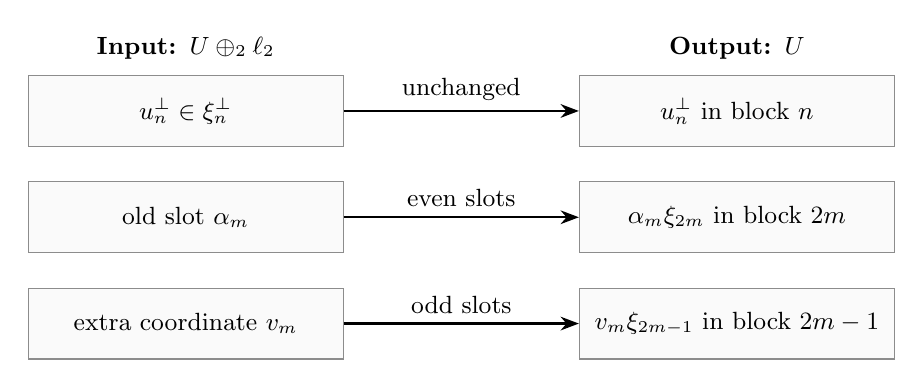
\begin{tikzpicture}[
 >=Stealth,
 box/.style={draw=black!45,minimum width=40mm,minimum height=9mm,
             align=center,fill=black!2},
 every node/.style={font=\small}]
 \node[box] (perpin) at (0,1.7) {$u_n^\perp\in\xi_n^\perp$};
 \node[box] (alphain) at (0,0.35) {old slot $\alpha_m$};
 \node[box] (vin) at (0,-1) {extra coordinate $v_m$};
 \node[box] (perpout) at (7,1.7) {$u_n^\perp$ in block $n$};
 \node[box] (evenout) at (7,0.35) {$\alpha_m\xi_{2m}$ in block $2m$};
 \node[box] (oddout) at (7,-1) {$v_m\xi_{2m-1}$ in block $2m-1$};
 \draw[->,thick] (perpin)--node[above]{unchanged}(perpout);
 \draw[->,thick] (alphain)--node[above]{even slots}(evenout);
 \draw[->,thick] (vin)--node[above]{odd slots}(oddout);
 \node[font=\small\bfseries] at (0,2.5) {Input: $U\oplus_2\ell_2$};
 \node[font=\small\bfseries] at (7,2.5) {Output: $U$};
\end{tikzpicture}

\caption{The frozen map \(L_\xi\). The perpendicular components and
the two scalar sequences form orthogonal coordinates. The picture
describes the frozen linear isometry; when the slots depend on the
input, it gives the pointwise norm identity but not preservation of
distances between distinct inputs.}
\label{fig:slots}
\end{figure}

\begin{lemma}
\label[lemma]{lem:frozen-inverse}
\(L_\xi:M\to U\) is an onto linear isometry. If \(y=(y_n)\in U\)
and \(\beta_n=\langle\xi_n,y_n\rangle\), its inverse is
\begin{equation}
\label{eq:frozen-inverse}
 (L_\xi^{-1}y)_{U_m}
 =y_m-\beta_m\xi_m+\beta_{2m}\xi_m,\qquad
 (L_\xi^{-1}y)_{V_m}=\beta_{2m-1}.
\end{equation}
\end{lemma}

\begin{proof}
All formulas are linear for fixed \(\xi\). Since
\(u_n^\perp\perp\xi_n\), the squared norm of \eqref{eq:frozen-map}
is
\begin{align*}
 \|L_\xi x\|^2
 &=\sum_n\|u_n^\perp\|^2+\sum_n|C_n|^2\\
 &=\sum_n\bigl(\|u_n\|^2-|\alpha_n|^2\bigr)
       +\sum_m|\alpha_m|^2+\sum_m|v_m|^2
 =\|x\|_M^2.
\end{align*}
This also proves the output belongs to \(U\).

For \(y\in U\), \(|\beta_n|\le\|y_n\|\), so
\((\beta_n)\in\ell_2\). The first two terms
\(y_m-\beta_m\xi_m\) in \eqref{eq:frozen-inverse} are perpendicular
to its last term. The prescribed vector therefore belongs to \(M\),
since
\begin{align*}
 &\sum_m\left(\|y_m-\beta_m\xi_m+\beta_{2m}\xi_m\|^2
                   +|\beta_{2m-1}|^2\right)\\
 &\qquad=\sum_m\bigl(\|y_m\|^2-|\beta_m|^2\bigr)
                 +\sum_m|\beta_{2m}|^2+\sum_m|\beta_{2m-1}|^2
 =\|y\|^2.
\end{align*}
For this input the old slot coefficient is \(\beta_{2m}\), and the
perpendicular component in block \(m\) is \(y_m-\beta_m\xi_m\).
The even and odd output slots consequently recover every \(\beta_n\),
so \eqref{eq:frozen-map} returns \(y\). This proves surjectivity and
the inverse formula.
\end{proof}

\subsection{What the moving slots must satisfy}

Given continuously differentiable unit-vector maps $w_n:M\to U_n$,
define $h(x)=L_{w(x)}x$. Explicitly,
\begin{equation}
\label{eq:h-formula}
 \begin{split}
 h(x)_n&=u_n+w_n(x)\bigl(C_n(x)-\langle w_n(x),u_n\rangle\bigr),\\
 C_{2m}(x)&=\langle w_m(x),u_m\rangle,
 \qquad C_{2m-1}(x)=v_m.
 \end{split}
\end{equation}
The frozen isometry shows that this is well-defined and gives
\begin{equation}
\label{eq:pointwise-norm}
 \|h(x)\|=\|x\|.
\end{equation}
This identity does not yet compare distinct inputs, whose slots may
differ. To control that difference, fix $c=1/100$ and define the
nonnegative weights
\begin{equation}
\label{eq:weights-radii}
 a_n(x)^2=\|u_n\|^2+\|u_{\lceil n/2\rceil}\|^2
                         +|v_{\lceil n/2\rceil}|^2.
\end{equation}
These weights follow the routing in \eqref{eq:h-formula}:
$|C_n(x)|\le a_n(x)$ and $\|u_n\|\le a_n(x)$, so the scalar
coefficient multiplying $w_n(x)$ has absolute value at most $2a_n(x)$.
We shall choose the slots so that
\begin{equation}
\label{eq:slot-budget}
 \sum_{n\ge1}a_n(x)^2\|Dw_n(x)\|^2\le c^2
 \qquad(x\in M).
\end{equation}
We shall show that each derivative of a finite approximant is within
$4c$ of a frozen isometry.

The second requirement concerns the coordinate supports. For every
finite family of distinct input points, we shall find neighborhoods
whose slots use disjoint coordinates in all sufficiently high blocks.
Indeed, the $n$th block of $D(x)=h(x)-u$ is a scalar multiple of
$w_n(x)$, so this separation gives the required local orthogonality
of $D$. We now choose the block dimensions and construct slots
satisfying both requirements.

\subsection{Finite stages and separating coordinates}

Choose a nonnegative smooth function $\psi:\R\to\R$ that is
positive on $(-1,1)$ and zero outside $[-1,1]$. For $k\ge1$, put
\[
 \mathcal A_k=\{-k,-k+1,\ldots,k\}^k.
\]
For $a=(a_1,\ldots,a_k)\in\mathcal A_k$, define
\[
 G_{k,a}(t)=\prod_{j=1}^k\psi(kt_j-a_j)
 \qquad(t\in[-1,1]^k).
\]
Every point of $[-1,1]$ is within $1/(2k)$ of some $a_j/k$ with
$-k\le a_j\le k$. Thus $G_k(t)=(G_{k,a}(t))_{a\in\mathcal A_k}$
is never zero on the cube. Its Euclidean norm has a positive minimum
there. Each factor $t\mapsto\psi(kt-a_j)$ is supported on an interval
of length $2/k$.

Give $U_n$ an orthonormal basis consisting of a single stage-zero
vector and a separate set of coordinates indexed by $\mathcal A_k$
for each $1\le k\le n$. Different stages are orthogonal. In
particular, we may take
\begin{equation}
\label{eq:block-dimensions}
 \dim U_n=1+\sum_{k=1}^n(2k+1)^k.
\end{equation}
From now on, use these blocks in the separable Hilbert spaces
\[
 U=\left(\bigoplus_{n\ge1}U_n\right)_2,
 \qquad V=\ell_2,\qquad M=U\oplus_2V
\]
on which the slots will be constructed. Enumerate the scalar
coordinates of $M$ and apply $\tanh$ to each of them. This gives
smooth Lipschitz functions $p_j:M\to[-1,1]$ that separate points.

Let $W_{n,0}$ be the constant stage-zero unit vector. For $1\le k\le n$,
let $W_{n,k}(x)$ be the vector supported on stage $k$ with coordinates
\begin{equation}
\label{eq:normalized-stage}
 W_{n,k}(x)_a
 =\frac{G_{k,a}(p_1(x),\ldots,p_k(x))}
        {\|G_k(p_1(x),\ldots,p_k(x))\|_2}.
\end{equation}
It is a smooth unit-vector map. Compactness of the cube, the positive
lower bound for the denominator, and boundedness of the derivatives
of the $p_j$ give
\[
 \sup_x\|DW_{n,k}(x)\|\le L_k<\infty.
\]
The same $L_k$ works for every $n\ge k$, since their stage-$k$
coordinate formulas are identical. Put $L_0=0$. No bound uniform in
$k$ is needed.

\subsection{A common budget for motion}

To obtain \eqref{eq:slot-budget}, use the tails of the weights
\eqref{eq:weights-radii} as nonnegative radii:
\[
 r_n(x)^2=\sum_{j\ge n}a_j(x)^2.
\]
Every input coordinate in the second and third terms of
\eqref{eq:weights-radii} is counted twice, so
\begin{equation}
\label{eq:radii-identities}
 r_1(x)^2=3\|u\|^2+2\|v\|^2,
 \qquad a_n(x)^2=r_n(x)^2-r_{n+1}(x)^2.
\end{equation}
Each $r_n$ is the norm of a bounded linear map into a Hilbert space.
It is $\sqrt3$-Lipschitz, smooth where positive, and tends to zero
at every fixed $x$.

With the fixed constant $c=1/100$, set
\begin{equation}
\label{eq:gamma}
 \gamma(r)=
 \begin{cases}
 \displaystyle\frac{c}{r\log(1/r)},&0<r<e^{-2},\\[4pt]
 0,&r\ge e^{-2}.
 \end{cases}
\end{equation}
This function is nonincreasing as $r$ increases. It has an infinite
first integral near zero but a finite weighted square integral:
\begin{equation}
\label{eq:gamma-integrals}
 \int_0^b\gamma(r)\,dr=\infty\quad(b>0),
 \qquad
 \int_0^\infty2r\gamma(r)^2\,dr
 =2c^2\int_2^\infty t^{-2}\,dt=c^2.
\end{equation}
The infinite first integral permits arbitrarily many rotations; the
second estimate will bound their total effect on the derivative.

Choose successive compact intervals $[a_k',b_k']\subset(0,e^{-2})$
for the transitions from stage $k-1$ to stage $k$, with
\[
 b_{k+1}'<a_k',\qquad b_k'<2^{-k},\qquad
 \gamma(r)/2\ge L_{k-1}+L_k\quad(0<r\le b_k').
\]
They can be chosen together with smooth nonincreasing angles
$\theta_k:[0,\infty)\to[0,\pi/2]$ such that
\begin{equation}
\label{eq:angle-bounds}
 \theta_k(r)=\pi/2\ (r\le a_k'),\qquad
 \theta_k(r)=0\ (r\ge b_k'),\qquad
 |\theta_k'(r)|\le\gamma(r)/(2\sqrt3),
\end{equation}
and the angles are constant near the interval endpoints. Here is a
direct construction. First choose $b_k'$ small enough for the
derivative bound and the preceding interval. By
\eqref{eq:gamma-integrals}, a sufficiently small $a_k'>0$ makes the
integral of $\gamma/(2\sqrt3)$ over $(a_k',b_k')$ larger than
$\pi/2$. A smooth nonnegative function supported inside this
interval, bounded above by $\gamma/(2\sqrt3)$ and with integral
larger than $\pi/2$, exists by approximation from below. Rescale it
to integral $\pi/2$ and integrate from $r$ to $+\infty$ to obtain
$\theta_k$.

For each $n$, define a unit-vector map $P_n(x,r)$ by following these
same timings through stages $0,\ldots,n$ and then stopping. On the
$k$th transition interval, $k\le n$, put
\[
 P_n(x,r)=\cos\theta_k(r)\,W_{n,k-1}(x)
            +\sin\theta_k(r)\,W_{n,k}(x).
\]
Between intervals use the intervening single stage; use $W_{n,0}$
above $b_1'$ and $W_{n,n}$ below $a_n'$, including at $r=0$.
Orthogonality of the stages makes this a unit vector. The endpoint
choices make $P_n$ continuously differentiable. On a transition,
\eqref{eq:angle-bounds} and the bounds for $L_k$ give
\begin{equation}
\label{eq:P-derivatives}
 \|\partial_xP_n(x,r)\|\le\gamma(r)/2,
 \qquad
 \|\partial_rP_n(x,r)\|\le\gamma(r)/(2\sqrt3)
 \qquad(r>0).
\end{equation}
Between transitions the first bound follows from monotonicity of
$\gamma$, and the second derivative is zero. Stage zero is constant,
so both bounds also hold where $\gamma=0$.

Set
\begin{equation}
\label{eq:moving-slot}
 w_n(x)=P_n(x,r_n(x)).
\end{equation}
Although $r_n$ need not be differentiable where it vanishes, $w_n$
is continuously differentiable there: in a neighborhood of any such
point, $r_n<a_n'$ and $w_n=W_{n,n}$. At a point with $r_n>0$,
the chain rule and \eqref{eq:P-derivatives} give
$\|Dw_n(x)\|\le\gamma(r_n(x))$. These slots satisfy the required
budget \eqref{eq:slot-budget}. Indeed, when $r_n>0$, monotonicity gives
\[
 (r_n^2-r_{n+1}^2)\gamma(r_n)^2
 \le\int_{r_{n+1}}^{r_n}2r\gamma(r)^2\,dr,
\]
and summing uses \eqref{eq:gamma-integrals}. When $r_n=0$, also
$a_n=0$, so that term in \eqref{eq:slot-budget} is zero.

The derivative budget controls metric distortion. We still need the
independent locality property that will make the free-space
linearization completely continuous.

\subsection{Local orthogonality of the slots}

\begin{lemma}
\label[lemma]{lem:slot-locality}
For every finite family of distinct points of $M$ there are
neighborhoods $O_j$ and an integer $l$ such that the coordinate
supports of $\{w_n(x):x\in O_j,\ n\ge l\}$ are disjoint for
different $j$.
\end{lemma}

\begin{proof}
For an empty family, take $l=1$ and the empty family of neighborhoods.
For a singleton, take $l=1$ and $O_1=M$.
In either case there is no disjointness condition to check.
Now consider two distinct points. Some $p_j$ has different values at them.
Choose $k_0\ge j$ sufficiently large and neighborhoods on which all
values of that $p_j$ on the two sides are separated by more than
$2/k_0$. At any stage $k\ge k_0$, a coordinate label that occurs on
both sides would require the $j$th factor $\psi(kp_j-a_j)$ to
be nonzero at points $x,y$ on opposite sides. Then both $p_j(x)$
and $p_j(y)$ would lie in $((a_j-1)/k,(a_j+1)/k)$, contradicting
$|p_j(x)-p_j(y)|>2/k_0\ge2/k$. Thus the unions of the supports on
the two neighborhoods are disjoint at every common stage
$k\ge k_0$.

Fix $0<\rho<a_{k_0}'$, below the completed transition into stage
$k_0$. Choose $l\ge k_0$ so that $r_l$ at each center is less than
$\rho/2$, and shrink both neighborhoods to have radius less than
$\rho/(2\sqrt3)$. Since $r_n\le r_l$ for $n\ge l$ and $r_l$ is
$\sqrt3$-Lipschitz, we have $r_n(x)<\rho$ throughout either
neighborhood whenever $n\ge l$. Only stages $k\ge k_0$ are then
active in $w_n(x)$. Distinct stages are orthogonal, and supports at
the same stage are disjoint by the first paragraph. This proves the
two-point assertion. For finitely many points, intersect the
neighborhoods obtained for every pair and take the largest cutoff.
\end{proof}

The use of small neighborhoods here is essential: pointwise decay of
the $r_n$ and their common Lipschitz bound suffice. Uniform decay on
bounded subsets of $M$ is neither claimed nor needed.

The constructed slots now satisfy both the derivative budget and
local separation. Use them in \eqref{eq:h-formula} to define $h$.
It remains to prove the two-point bounds and surjectivity; the
pointwise norm identity alone does not give either conclusion.

\subsection{Finite approximants and global inverses}

Let $h_N$ be the same rearrangement with slots
\[
 w_n^{(N)}(x)=
 \begin{cases}w_n(x),&n\le N,\\W_{n,0},&n>N.\end{cases}
\]
Let $A_0$ denote the isometry with all slots equal to $W_{n,0}$.
Only output blocks $n\le2N$ of $h_N-A_0$ can be nonzero, and their
formulas are continuously differentiable. Thus $h_N$ is a
continuously differentiable map between Hilbert spaces. It also
satisfies $\|h_N(x)\|=\|x\|$.

\begin{lemma}
\label[lemma]{lem:approximant-inverse}
Each $h_N:M\to U$ is a continuously differentiable bijection with
continuously differentiable inverse, and
\begin{equation}
\label{eq:hN-bounds}
 (1-4c)\|x-x'\|\le\|h_N(x)-h_N(x')\|
             \le(1+4c)\|x-x'\|.
\end{equation}
\end{lemma}

\begin{proof}
Fix a point and a unit direction, and abbreviate the approximant slots
$w_n^{(N)}(x)$ and their directional derivatives by $w_n,\dot w_n$;
the slots with $n>N$ have derivative zero. Differentiating the inputs in
\eqref{eq:h-formula} with the slots frozen gives the onto isometry
$L_{w^{(N)}(x)}$. The remaining terms in output block $n$ are
\[
 \dot w_n(C_n-\langle w_n,u_n\rangle)
 +w_n\bigl(\dot C_n-\langle\dot w_n,u_n\rangle\bigr),
 \qquad
 \dot C_{2m}=\langle\dot w_m,u_m\rangle,
 \quad \dot C_{2m-1}=0.
\]
Put $R^2=\sum_n a_n(x)^2\|\dot w_n\|^2\le c^2$. Since
$|C_n-\langle w_n,u_n\rangle|\le2a_n$, the first term has
Hilbert norm at most $2R$. Each of the scalar sequences
$(\dot C_n)_n$ and $(\langle\dot w_n,u_n\rangle)_n$ has
$\ell_2$ norm at most $R$, because $a_n\ge\|u_n\|$.
Therefore
\begin{equation}
\label{eq:derivative-perturbation}
 \|Dh_N(x)-L_{w^{(N)}(x)}\|\le4c.
\end{equation}
A Neumann-series perturbation of the isometry gives
\begin{equation}
\label{eq:derivative-bounds}
 \|Dh_N(x)\|\le1+4c,
 \qquad \|Dh_N(x)^{-1}\|\le(1-4c)^{-1}.
\end{equation}

We next establish global bijectivity before using the lower
Lipschitz estimate. Put $F_N=\bigoplus_{n\le2N}U_n$ and let $P$
project onto $F_N^\perp$. We have
\[
 Ph_N=PA_0.
\]
For a fixed $b\in F_N^\perp$, the map $h_N$ thus restricts to
\begin{equation}
\label{eq:fiber-map}
 A_0^{-1}(b)+A_0^{-1}(F_N)\longrightarrow b+F_N.
\end{equation}
These affine spaces have the same finite dimension. The derivative
is an isomorphism between their tangent spaces. Indeed it maps
$A_0^{-1}(F_N)$ into $F_N$; conversely, for $z\in F_N$, the vector
$t=Dh_N(x)^{-1}z$ satisfies
$PA_0t=PDh_N(x)t=0$. Thus \eqref{eq:fiber-map} is a local
diffeomorphism. It is proper, since an inverse image of a compact
set is closed and norm-bounded by $\|h_N(x)\|=\|x\|$, hence compact
in this finite-dimensional source fiber.

A proper local diffeomorphism between affine Euclidean spaces of
the same dimension is bijective. To recall the topological argument,
its image is open by local invertibility and closed by properness,
so it is the entire target. Each fiber is compact and discrete,
hence finite. Local inverse neighborhoods, together with properness
to exclude further preimages nearby, make it a covering map. A
covering of a simply connected Euclidean space with connected
source has one sheet. Applying this to \eqref{eq:fiber-map} proves
that $h_N$ is bijective on each fiber and therefore on all of $M$.

The local inverses supplied by the inverse function theorem agree
and form a global continuously differentiable inverse. Integrating
the two bounds in \eqref{eq:derivative-bounds} along line segments,
for $h_N$ and for its now-defined inverse, proves
\eqref{eq:hN-bounds}.
\end{proof}

\subsection{Passing to an onto limit}

\begin{proof}[Completion of the proof of Theorem~\ref{thm:hilbert-map}]
For fixed \(x=(u,v)\), the first \(N\) output blocks of \(h_N(x)\)
and \(h(x)\) agree. Indeed, their own slots agree in those blocks,
and the old slot used in an even block \(2m\le N\) has \(m\le N\).
For either list \(\zeta=w(x)\) or \(\zeta=w^{(N)}(x)\), write
\[
 C_{2m}^{\zeta}=\langle\zeta_m,u_m\rangle,\qquad
 C_{2m-1}^{\zeta}=v_m.
\]
Then
\((L_\zeta x)_n-u_n
 =\zeta_n(C_n^\zeta-\langle\zeta_n,u_n\rangle)\).
Since \(|C_n^\zeta|\le a_n(x)\) and \(\|u_n\|\le a_n(x)\),
each difference from \(u_n\) has norm at most \(2a_n(x)\).
For the remaining blocks, the difference between the two maps has
norm at most \(4a_n(x)\). Hence
\begin{equation}
\label{eq:h-pointwise-limit}
 \|h_N(x)-h(x)\|
 \le4r_{N+1}(x)\longrightarrow0.
\end{equation}
For fixed \(x,x'\), take \(N\to\infty\) in
\eqref{eq:hN-bounds}. This proves the two-sided bounds
\eqref{eq:h-bounds}, since \(1-4c=24/25\) and
\(1+4c=26/25\). In particular, \(h\) is injective. It fixes zero by
\eqref{eq:pointwise-norm}.

We now prove surjectivity. Fix \(y=(y_n)\in U\) and, using
\Cref{lem:approximant-inverse}, put
\[
 x_N=h_N^{-1}(y).
\]
Freeze the slots of \(h_N\) at this particular input:
\[
 \xi_n^{(N)}=w_n^{(N)}(x_N),\qquad
 \beta_n^{(N)}=\langle \xi_n^{(N)},y_n\rangle.
\]
The directions may vary with \(N\). Nevertheless
\(y=L_{\xi^{(N)}}x_N\) is an exact equality for each \(N\), so
\Cref{lem:frozen-inverse} gives
\begin{equation}
\label{eq:xN-inverse}
 (x_N)_{U_m}
 =y_m-\beta_m^{(N)}\xi_m^{(N)}
       +\beta_{2m}^{(N)}\xi_m^{(N)},\qquad
 (x_N)_{V_m}=\beta_{2m-1}^{(N)}.
\end{equation}
The component \(y_m-\beta_m^{(N)}\xi_m^{(N)}\) is perpendicular
to \(\xi_m^{(N)}\). Thus its squared norm is
\(\|y_m\|^2-|\beta_m^{(N)}|^2\), and the last term in the
\(U_m\) formula adds orthogonally.

For every integer \(s\ge1\), it follows that
\begin{align}
\label{eq:inverse-tail}
 &\sum_{m\ge s}
   \left(\|(x_N)_{U_m}\|^2+|(x_N)_{V_m}|^2\right)\notag\\
 &\quad=\sum_{m\ge s}
   \left(\|y_m\|^2-|\beta_m^{(N)}|^2
               +|\beta_{2m}^{(N)}|^2
               +|\beta_{2m-1}^{(N)}|^2\right)\notag\\
 &\quad=\sum_{n\ge s}\|y_n\|^2
                -\sum_{n=s}^{2s-2}|\beta_n^{(N)}|^2
 \le\sum_{n\ge s}\|y_n\|^2.
\end{align}
Here \(|\beta_n^{(N)}|\le\|y_n\|\), so all squared-coefficient
series converge. The last equality is exact: the even and odd
indices \(2m,2m-1\) for \(m\ge s\) partition the integers
\(n\ge2s-1\); their sum cancels that tail of
\(\sum_{n\ge s}|\beta_n^{(N)}|^2\). The only uncancelled negative
terms have \(s\le n\le2s-2\). This finite sum is empty when \(s=1\).
Keeping it is what avoids double counting the output's perpendicular
and slot components.

The right side of \eqref{eq:inverse-tail} tends to zero with \(s\),
independently of \(N\). At \(s=1\) the equality gives
\(\|x_N\|=\|y\|\). For each \(s\), the heads
\[
 \bigl((x_N)_{U_m},(x_N)_{V_m}\bigr)_{m<s}
\]
lie in a bounded subset of the finite-dimensional space
\(\bigoplus_{m<s}(U_m\oplus\R)\). By successive subsequence
selection in these finite-dimensional spaces and a diagonal choice,
there is an increasing sequence \(N_j\) for which every fixed head
converges.

This diagonal subsequence is Cauchy in the full norm. Given
\(\epsilon>0\), choose \(s\) so that
\(\sum_{n\ge s}\|y_n\|^2<(\epsilon/4)^2\). By
\eqref{eq:inverse-tail}, the tail of each of \(x_{N_j}\) and
\(x_{N_k}\) has norm less than \(\epsilon/4\).
For sufficiently large \(j,k\), convergence of the fixed head makes
its difference smaller than \(\epsilon/2\). The triangle inequality
then gives \(\|x_{N_j}-x_{N_k}\|<\epsilon\).
Completeness of \(M\) yields \(x_{N_j}\to x\) in norm for some
\(x\in M\).

Finally, apply the pointwise convergence estimate at this fixed
limit \(x\), and use the common upper Lipschitz bound for \(h_{N_j}\):
\begin{align*}
 \|h(x)-y\|
 &\le\|h(x)-h_{N_j}(x)\|
      +\|h_{N_j}(x)-h_{N_j}(x_{N_j})\|\\
 &\le4r_{N_j+1}(x)+(1+4c)\|x-x_{N_j}\|\longrightarrow0.
\end{align*}
Thus \(h(x)=y\). Since \(y\) was arbitrary, \(h\) is onto.

The local orthogonality asserted in the theorem follows from
\Cref{lem:slot-locality}. For its neighborhoods $O_j$ and cutoff $l$,
let $H_j$ be the closed span of the union of coordinate supports of
$w_n(x)$ with $x\in O_j$ and $n\ge l$. These are mutually orthogonal
coordinate subspaces of $U_{\ge l}$. Each block $D(x)_n$ is a scalar
multiple of $w_n(x)$ by \eqref{eq:h-formula}. Its convergent tail
therefore belongs to $H_j$ for every $x\in O_j$, because $H_j$ is closed.
This verifies exactly \eqref{eq:local-orthogonality} and completes the proof.
\end{proof}

\section{The counterexample}
\label{sec:assembly}

The Hilbert construction supplies the geometric hypotheses of localized
linearization. The resulting completely continuous operator then meets
the weighted graph criterion.

\begin{proof}[Proof of \Cref{thm:main}]
Take the real Hilbert spaces \(U\), \(V=\ell_2\), \(M=U\oplus_2V\)
and the map \(h:M\to U\) from \Cref{thm:hilbert-map}. The blocks
\(U_n\) are finite dimensional, so \(U\) and \(M\) are separable;
as Hilbert spaces they are complete. Put
\[
 E=\F(M),\qquad D=h-\pi_U,\qquad q=\widehat D:E\to U.
\]
The map \(D\) is Lipschitz, \(D(0)=0\), and it has the finite-family
tail-coordinate orthogonality required by
\Cref{thm:localized-linearization}. That theorem makes \(q\)
completely continuous. By \eqref{eq:linearization} and
\eqref{eq:h-bounds},
\[
 \|q\|=\Lip(D)\le\Lip(h)+\|\pi_U\|
 \le\frac{26}{25}+1=\frac{51}{25}.
\]
Set
\[
 Q_1:E\oplus_1\ell_2\to M,\qquad Q_1(e,v)=(qe,v),\qquad
 X=Z_{Q_1},\qquad Y=Z_q.
\]
All hypotheses of \Cref{prop:criterion} hold with
\(a=24/25\), \(b=26/25\). It supplies the coordinatewise bijection
\(\Psi:X\to Y\), an isometric copy of \(c_0(\ell_2)\) in \(X\),
and exclusion of every linearly isomorphic copy from \(Y\).
In particular \(X\) and \(Y\) are not linearly isomorphic.

Since \(L_q\le51/25\) and \(K_q=\max\{L_q,1\}\le51/25\),
\eqref{eq:criterion-bounds} gives
\[
\begin{aligned}
 \Lip(\Psi)&\le
 \max\left\{1+\frac{51}{25},\frac{26}{25}\right\}
 =\frac{76}{25},\\
 \Lip(\Psi^{-1})&\le
 \max\left\{1+\frac{2(51/25)}{24/25},\frac{25}{24}\right\}
 =\frac{21}{4}.
\end{aligned}
\]
The latter inequality is equivalent to the lower bound
\(\|\Psi(s)-\Psi(t)\|_Y\ge(4/21)\|s-t\|_X\).
Both bounds hold for all pairs \(s,t\in X\), exactly as in
\eqref{eq:main-bounds}.
\end{proof}


\bibliographystyle{plain}
\bibliography{references}
\end{document}
